Many researchers have done to improve stance detection accuracy. Different ideas and architectures have been applied. In the following part, previous research and papers have been overviewed.  

In 2016 \cite{Augenstein2016StanceDW} started working on the challenging task without assuming neither target is clearly mentioned in the text nor training date is given for every target. Their dataset construct of tweets mostly containing politicians and popular issues. The paper mainly focuses on detecting a stance with respect to unseen targets. \cite{Augenstein2016StanceDW} used conditional LSTM encoding on Tweeter data. \cite{Augenstein2016StanceDW} inferred that using unconditional LSTM has the best performance for unseen targets. Their results are improved by using bidirectional encoding. Using LSTM-based models lead to better results than Majority class, SVM (\cite{svc}), and BoW (\cite{bow}) as baselines in this experiment.

\cite{UCLMR} has developed an end-to-end stance detection system including lexical and similarity-based features which is passed through a multi-layer perception model. UCLMR's\footnote{UCL Machine Reading} model claimed third place in FNC-1\footnote{First stage of a competition Fake News Challenge(FNC-1) is exploring how artificial intelligence technologies could be leveraged to combat fake news\footnote{fakenewschallenge.org}. Numerous researchers has interest in this field and many papers has published besides this challenge.}. The model architecture is illustrated in Figure \ref{fig:UCLMR-system}. Headline and body texts are tokenized by scikit-learn\footnote{\cite{sikit-learn}}. Furthermore, \cite{UCLMR} used both term frequency (TF) vector of headline and claim and cosine similarity between head and body, and $l$2-normalized TF-IDF vectors. Besides, stop words are excluded. \cite{UCLMR} achieved FNC-1 score of 75.20\% on the test data set.
\begin{figure}
	\centering
	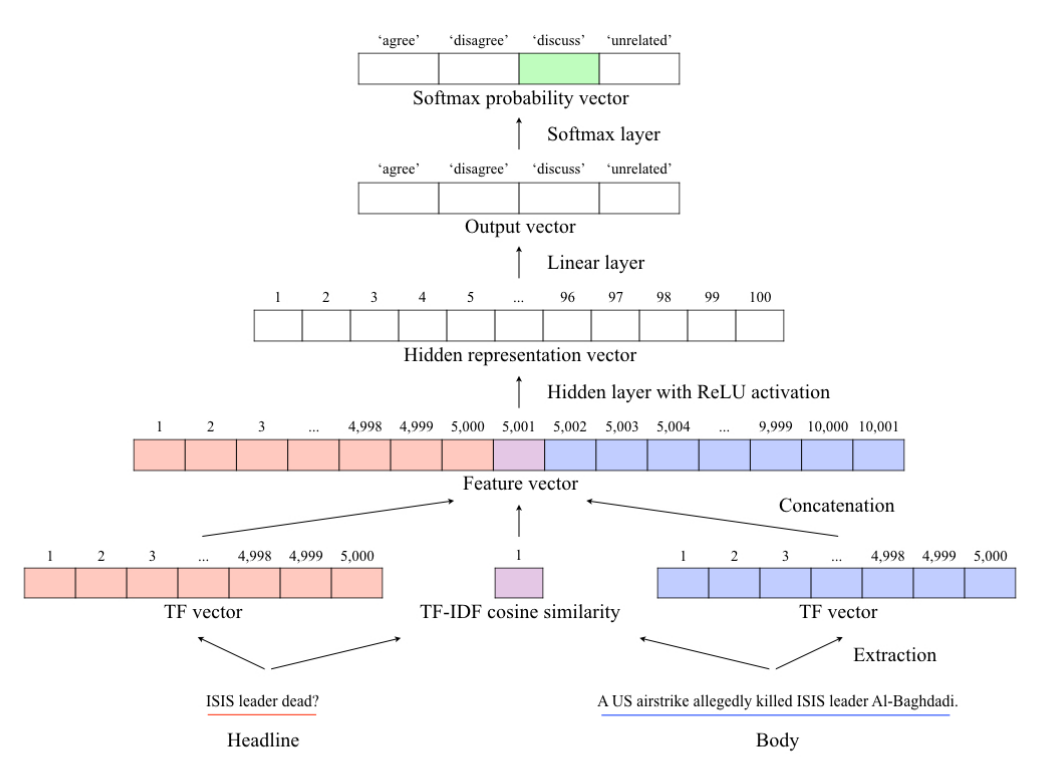
\includegraphics[scale=0.4]{statistics/stance/simple-baseline-FNC.png}
	\caption{Schematic diagram of UCLMR’s system.}
	\label{fig:UCLMR-system}
\end{figure}


\cite{Hierarchical-Attention-Network} have mainly focused on linguistic information such as polarity and argument of each document to represent a document. As shown in figure \ref{fig:hierarchical_att} document, sentiment, dependency, and argument representations are used in model architecture. \cite{Hierarchical-Attention-Network} concluded that every linguistic information with attention mechanism improves stance detection, And using linguistics features altogether outperform using them individually. More details are provided below.

\begin{itemize}
	\item \textbf{Document Representation}: \cite{Hierarchical-Attention-Network} used a LSTM model to represent each document.
	\item \textbf{Sentiment Representation}: As sentiment representation, an LSTM model is used to learn the representation of sentiment information. The sentimental word sequence of each document is extracted from sentiment lexicon. 
	\item \textbf{Dependency Representation}: This feature is used to capture inter-word relationships. Firstly, relations from the dependency parser are extracted. Then, representation of dependency sequence is learnt by using an LSTM layer.
	\item \textbf{Argument Representation}: The argument is considered as the author's stance. \cite{Hierarchical-Attention-Network} used a binary classification to detect the document's argument sentence. Then, it learned the sequence representation of word sequence in argument sentences by making use of LSTM layer.
\end{itemize}

In addition, it utilized a hierarchical attention network in order to weigh the importance of linguistic information, and learn the mutual attention between the document and linguistic information. \cite{Hierarchical-Attention-Network} mentioned that the Hyper Attention layer in Figure \ref{fig:hierarchical_att}, had a considerable influence on model performance. 

\begin{figure}
	\centering
	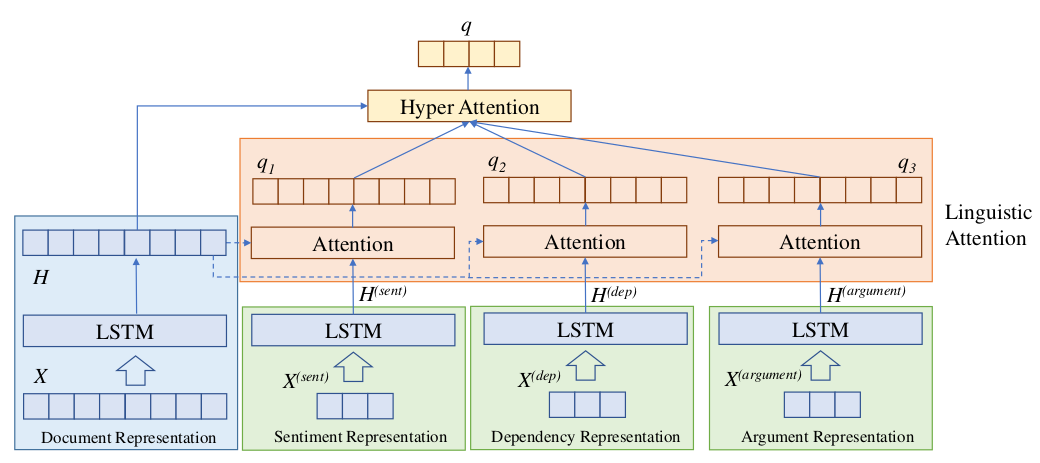
\includegraphics[scale=0.4]{statistics/stance/hierarchial-attention-network.png}
	\caption{Overview of \cite{Hierarchical-Attention-Network} model.}
	\label{fig:hierarchical_att}
\end{figure}

\cite{memory_network} present a novel end-to-end memory network in 2018 to predict stance and extract snippet of the prediction. The proposed model mainly focuses on relevant paragraphs. This model incorporates recurrent, convolutional neural networks and similarity matrixes. \cite{memory_network} mentioned that detecting \textit{Disagree} is the hardest label to predict. To overcome the imbalance issue, \cite{memory_network} select the same number from each class in each iteration. 
\begin{figure}
	\centering
	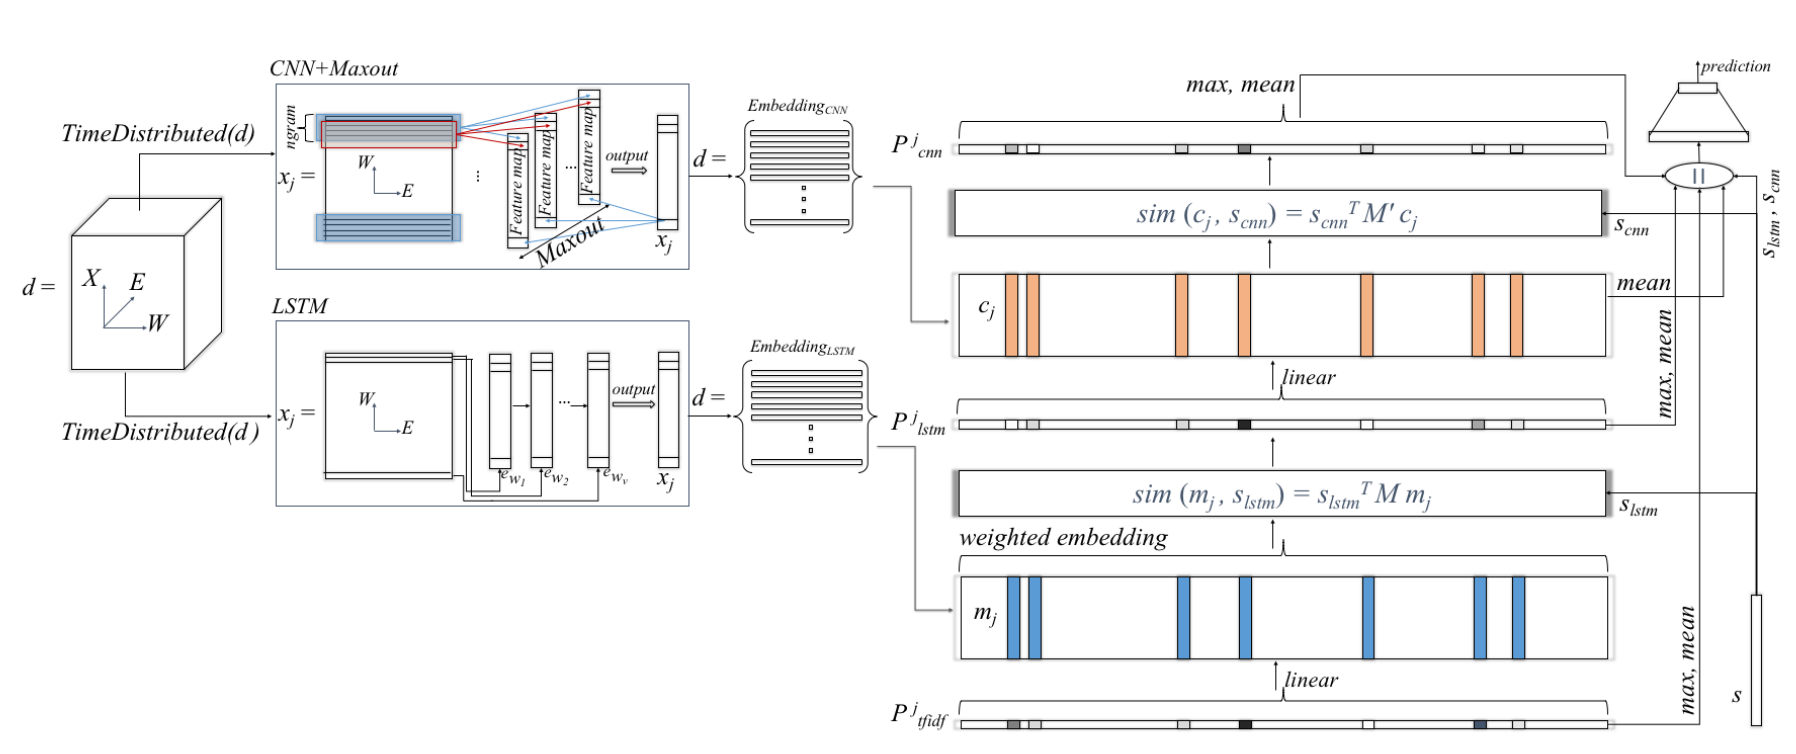
\includegraphics[scale=0.25]{statistics/stance/memoty_network.png}
	\caption{Architecture of Memory Network for the stance classification task.}
	\label{fig:mem_network}
\end{figure}

\cite{stance_robust} mainly focused on the robustness of a stance detection classifier. Trained models  on a single data set in a special domain, won't be robust enough on other domains. So they suggested using a multi-domain dataset or use multi-dataset learning methods to improve model generalization. The model architecture is constructed of fine-tuned BERT\cite{bert} and a single dense classifier at the top. \cite{stance_robust} used 5 fixed seed values during training and reported averaged results of trained models. \cite{stance_robust} concluded that MDL(multi-dataset learning) has a significant impact on increasing model robustness.
